\documentclass[11pt,a4paper]{article}
%% Packages élémentaires %%
\usepackage[utf8]{inputenc}
\usepackage{mathpazo,etoolbox, graphicx, wrapfig, pbox, fancybox, hyperref, appendix, geometry, amsmath, amssymb, tikz, pgfplots, calc, enumitem, colortbl, subfiles}
\usepackage{forest} % Pour une arborescence de fichiers
%% supression des alineas
\setlength{\parindent}{0pt}

%% Ajustement des marges
\geometry{hmargin=2.4cm, vmargin = 2.1cm}

%% Changement des "---" en "--" dans itemize
\setlist[itemize]{itemsep=10pt, label={--}}

%% Couleurs %%
\usepackage{xcolor}
\definecolor{bleu}{RGB}{14, 68, 175}
\definecolor{BGbleu}{RGB}{222, 233, 255 }
\definecolor{BGorange}{RGB}{255, 216, 154}
\definecolor{rouge}{RGB}{201, 0, 0}
\definecolor{vert}{RGB}{14, 137, 0}
\definecolor{BGgris}{RGB}{222,230,230}

% Couleurs additionnelles jolies
\definecolor{vertPale}{RGB}{227, 255, 233}
\definecolor{bleuPale}{RGB}{232, 238, 255}
\definecolor{jaunePale}{RGB}{253, 255, 189}
\definecolor{orangePale}{RGB}{255, 223, 189}
\definecolor{rougePale}{RGB}{255, 217, 217}
\definecolor{mauvePale}{RGB}{249, 222, 255}

\newcommand\rouge[1] {{\color{rouge}{#1}}}
\newcommand\bleu[1] {{\color{bleu}{#1}}}
\newcommand\term[1] {\textbf{{\color{bleu}{#1}}}}
\newcommand\green[1]{{\color{vert}{#1}}}
\newcommand\folder[1]{\green{{#1}}}
\newcommand\subfolder[1]{\bleu{{#1}}}

%% Checkbox : https://tex.stackexchange.com/questions/16000/creating-boxed-check-mark
\newcommand{\checked}{$\mbox{\ooalign{$\checkmark$\cr\hidewidth$\square$\hidewidth\cr}}$}
\newcommand{\unchecked}{$\square$}
%% Cadres %%

\newcommand{\custombox}[4]{
    \fcolorbox{#4}{#1}{\parbox{#2\linewidth}{ 
    #3
    }}
}

\newcommand{\presentationBox}[3]{
    \custombox{#2}{0.45}{
        \begin{center}
            #1
        \end{center}
        \begin{small}
            \textit{#3}
        \end{small}
    }{white}    
}
\setlength{\fboxsep}{1em} % espace entre le bord d'une boite et le texte dedans

\newcommand\bbm[1]{
\begin{center}
    \fcolorbox{black}{BGbleu}{\parbox{\linewidth}{ 
    #1
    }}
\end{center}
}


\newcommand\bo[1]{
\begin{center}
\fcolorbox{black}{BGorange}{\parbox{\textwidth}{ 
#1
}}
\end{center}}

\newcommand\bb[1]{
\begin{center}
\fcolorbox{black}{BGbleu}{\parbox{\textwidth}{ 
\begin{Large}
\begin{center}
#1
\end{center}
\end{Large}
}}
\end{center}}


\newcommand\boite[1]{
\begin{center}
\fbox{\parbox{\textwidth}{ \begin{center}
\begin{Large}
#1
\end{Large}
\end{center}}}
\end{center}}

\newcommand\aparte[1]{
\begin{center}
\fcolorbox{white}{BGgris}{\parbox{\linewidth}{ \textit{A parte} \\
#1 }}
\end{center}}
\newcommand\bg[2]{
\begin{center}
\fcolorbox{white}{BGgris}{\parbox{\linewidth}{ \textit{#1} \\
#2 }}
\end{center}}

\newcommand\exemple[1]{
\begin{center}
\fcolorbox{white}{BGgris}{\parbox{\linewidth}{ \textit{Exemple} \\
#1 }}
\end{center}}

%% Commandes %%
\newcommand\imp[1]{\underline{\textbf{#1}}}
\newcommand\eq[1]{\begin{large}
\begin{align*}
#1
\end{align*}
\end{large}}
%% Commandes fantaisistes (cf. Internet) %%
\renewcommand{\parallel}{ \mathbin{\!/\mkern-5mu/\!} }
\newcommand{\q}[1]{{%
\font\larm = larm1000%
\larm%
\char 190}{ \textit{#1} }{%
\font\larm = larm1000%
\larm%
\char 191}}

%% Wrapping %%
\newcommand\wrap[4]{\begin{wrapfigure}[#1]{#2}{#3\textwidth}
#4
\end{wrapfigure}}



%% Code %%
\usepackage{listings}
\definecolor{codegreen}{rgb}{0,0.6,0}
\definecolor{codegray}{rgb}{0.5,0.5,0.5}
\definecolor{codepurple}{rgb}{0.58,0,0.82}
\definecolor{backcolour}{RGB}{242,242,242}
\definecolor{codeorange}{RGB}{255,140,0}

\newcommand{\code}[1]{\texttt{{\color{codepurple}{#1}}}}
\newcommand{\codep}[1]{\texttt{{\color{codegreen}{#1}}}}

\lstdefinestyle{mystyle}{
    backgroundcolor=\color{backcolour},   
    commentstyle=\color{bleu},
    keywordstyle=\color{codeorange},
    numberstyle=\tiny\color{codegray},
    stringstyle=\color{codepurple},
    basicstyle=\ttfamily\footnotesize,
    breakatwhitespace=false,         
    breaklines=true,                 
    captionpos=b,                    
    keepspaces=true,                 
    numbers=left,                    
    numbersep=5pt,                  
    showspaces=false,                
    showstringspaces=false,
    showtabs=false,                  
    tabsize=2
}

\lstset{style=mystyle}
\lstset{language=C}

\lstdefinestyle{cppstyle}{
basicstyle=\footnotesize\sffamily\color{black},
commentstyle=\color{mygray},
frame=single,
numbers=left,
numbersep=5pt,
numberstyle=\tiny\color{mygray},
keywordstyle=\color{mygreen},
showspaces=false,
showstringspaces=false,
stringstyle=\color{myorange},
tabsize=2
}


%% Leftbar (merci M. Albrecht-Marc)
\usepackage{framed}

\renewenvironment{leftbar}[1][\hsize]
{%
     \def\FrameCommand
     {%
         {\color{black}\vrule width 3pt}%
         \hspace{7pt}%must no space.
        % \fboxsep=\FrameSep\colorbox{yellow}%
     }%
     \MakeFramed{\hsize#1\advance\hsize-\width\FrameRestore}%
}
{\endMakeFramed}
\newenvironment{blueleftbar}[1][\hsize]
{%
     \def\FrameCommand
     {%
         {\color{blue}\vrule width 3pt}%
         \hspace{7pt}%must no space.
        % \fboxsep=\FrameSep\colorbox{yellow}%
     }%
     \MakeFramed{\hsize#1\advance\hsize-\width\FrameRestore}%
}
{\endMakeFramed}

\usepackage[english]{babel}

\usepackage{etoolbox}

\providetoggle{darkmode}
\settoggle{darkmode}{false}


\iftoggle{darkmode}{
    \pagecolor{black}
    \color{white}
    }

\usepackage{array, algorithm, algpseudocode}



% Scientia Vincere Tenebras
\usepackage{graphicx}
\usepackage{transparent}
\usepackage{eso-pic}
\newcommand\BackgroundPic{
    \put(0,0){
        \parbox[b][\paperheight]{\paperwidth}{
            \vfill
            \centering
            {\transparent{0.1}
\includegraphics[width=1.1\textwidth]{SVT.png}}
            \vfill
        }
    }
}


\begin{document}
\thispagestyle{empty}
\pagenumbering{Roman}

%page de titre
\begin{center}
\AddToShipoutPicture*{\BackgroundPic}
\end{center}
\begin{figure}[h!]
    \begin{center}
    
\includegraphics[scale=0.6]{EPB.png}
    \end{center}
    \end{figure}

\begin{center}
\begin{LARGE}
\textbf{Techniques of artificial intelligence}
\end{LARGE}
\end{center}
\vspace{2mm}
\begin{center}
\begin{large}
PROJ-H418
\end{large}
\end{center}


\vspace{4mm}
\begin{center}\bf\huge
\rule{16cm}{2pt}\\
\bigskip
{Project report : \textit{Monte-Carlo} tree-search for Checkers}
\rule{16cm}{2pt}
\end{center}

\vfill

\begin{minipage}[t]{0.4\textwidth}
\begin{flushleft}
    \large{Sami \textsc{Abdul Sater}} \\
    \large{Alexandre \textsc{Flachs}} \\
    \large{Diego \textsc{Rubas}} \\
    \large{Jeanne \textsc{Szpirer}} \\
\end{flushleft}

\end{minipage}

\vfill
\begin{center}
Academic year 2021-2022
\end{center}

\newpage
\tableofcontents

\pagenumbering{arabic}

%%%%%%%%%%%%%%%%%

\section{Introduction : \textit{Monte-Carlo} tree-search}
Tree search is an intuitive way to solve a game with a limited number of possible moves. A \textit{Monte-Carlo} tree-search (MCTS) is a tree-search algorithm that exploits \textbf{randomness} and \textbf{evaluation of simulated games} to decide the next move. The tree is built according to a policy that we hereby define.\\

Repeat $n_{\text{iter}}$ times :
\begin{enumerate}
    \item \textbf{Selection} of the \textbf{best} node according to policy
    \begin{itemize}[label=$\blacktriangleright$]
        \item \textbf{Expansion} of nodes if needed
    \end{itemize}
    \item \textbf{Simulation} of the rest of the game, starting from the selected node. This simulation ends with a \textbf{reward} that takes into account if the game has been won or not.
    \item This reward is \textbf{backpropagated} to the selected node.
\end{enumerate}
Once all the simulations have been done, the tree is considered to be computed (though not necessarily fully expanded) : we then select the \textbf{best child}.\\

\subsection{Parameters}
Are variable :
\begin{itemize}
    \item The selection policy
    \item The best-child selection policy
    \item The number of iterations
\end{itemize}

\subsection{Optimization and constraints}
There are no particular mathematical constraints to ensure for this project. However, constraints are to be imposed to make it sure it runs in a \textbf{realistic time}, e.g. 15 seconds by move. \\

Under this time, the parameters of the search ($n_{\text{iter}}$, the policies, and more) must be tuned to \textbf{optimize the win rate}. \\

This report presents the implementation of a MCTS on top of a Checkers game. Explaining first the rules, very briefly, we then explain the implementation itself before presenting results of our AI agains a \textbf{deterministic} AI (minimax).

\subsection{Our contribution}
We took the implementation of a Checkers game with a minimax AI on top of it from an Open Source repository. Implementing MCTS required a huge refactor, at the game level and thus also at the minimax level. After implementing MCTS and refactoring, a benchmark was run for different parameters, which lead to an optimization of the win rate over the parameters of the search.
\section{Rules of the Checkers game}
Let's briefly go through the rules of Checkers game. Particular terms will be used and highlighted, that will be important for the algorithm. \\

The game opposes two adversary, here named \code{RED} and \code{WHITE}, and consists of a \term{board} and \term{pieces} on it, each belonging to one player. Each piece then has a color, and the board has pieces on it. Here are some additional information :
\begin{itemize}[label=$\blacktriangleright$]
    \item A board can call a function to get all the pieces of a certain color
    \item It is possible to move a piece of the board using a \code{move} function
    \item A piece has a defined \term{position} $(x,y)$ where $x$ denotes the row and $y$ the column of the piece. A piece is hence defined by a color and its position : $P = (C, x, y)$
\end{itemize}

\subsection{Beginning of the game}
Each player has 12 pieces, that begin at the same position for every game, and the starting position is the conventional position for Checkers game. From here, the \code{WHITE} begins (by convention) and can perform a move.
\subsection{Movements}
In this section, we define with words how a player can move a piece. We could define it in an algorithmic way, but this wouldn't be particularly relevant for the sake of this report. \\

A player can only \term{move} a piece in diagonal, going forward, and can move only one row forward, unless an ennemy piece is on its way. In this case, if the piece can reach a place on the board and some enemy pieces are on its way, the enemy pieces are discarded and the initial piece can find its final destination. We say that the pieces has \term{skipped} $n$ pieces if $n$ enemy pieces were discarded. \\

If a piece reaches the opposite side of the board, it becomes a \term{queen} and can from now on move backwards.
\subsection{Endgame}
A game ends when
\begin{itemize}
    \item a player has no pieces left : the adversary wins ;
    \item all remaining pieces are queens and no piece was discarded in the last 20 moves : it ends as a draw.
\end{itemize}


\section{Implementation of MCTS to Checkers}
To implement the tree search, we need to define a tree and the policies associated to the search. Each time the AI has to play, it calls the algorithm, beginning to build the tree (as described in the introduction). Once the tree is built, it selects the best move according to a policy that will be described further.

\subsection{Nodes}
A node in the tree corresponds to
\begin{itemize}
    \item The parent node
    \item A \term{state} of the game : a \code{board} element
    \item The move that lead from previous node to this one (\textit{parent action}) : a \code{move} element
    \item \code{visits} : number of times that this node was visited during the search
    \item \term{reward} : number of times that this node led to victory
\end{itemize}
When the AI is instanciated, the root node has no parent and no parent action, \code{visits} is set to 1 and \code{reward} is set to 0. \\

The resulting constructor for the class \code{MCNode} can be found on listing \ref{listing:constructor}.

\subsection{Selection policy}
To select a child node from which perform a simulation, the current node first needs to check if it has children, and if so, if all children have been explored. That is, the current node builds a list of possible children (resulting from the possible moves) and looks for children that are not currently in the tree. \\

Thus, if the node is currently not \term{fully explored}, we \term{expand} the current node. If the node is fully explored, we select the \term{best child} to perform the simulation. \\

Intuitively, if there is a sequence of fully explored nodes that leads to a leaf, this will be the privileged path. Otherwise, the algorithm will return the first created child node of a non-fully-explored node. This yields in listing \ref{listing:selection}.

\subsection{Expansion}
When a node $N$ needs to be extended, first a list of possible moves is created. Then, a \rouge{random move $r$ is drawn}\footnote{pour l'instant. a modifier si on change} and a node $N_r$ is created from this move, having $N$ as \term{parent node} and $r$ as \term{parent action}. This yields in listing \ref{listing:expand}.
\subsection{Best child policy}
There are multiple calls to the best-child policy :
\begin{itemize}
    \item When the tree is built and we need to perform an actual choice : we choose the best child node of the root node 
    \item During the selection, when a node is fully explored and we need to go down a level to look for a leaf node to select or a node to expand. \\
\end{itemize}

During the exploration of the tree, the attributes \code{reward} and \code{visits} of each node are updated, such that at any time, it is possible to define, for each node, a value evaluating the node. We chose the following values\footnote{Insérer source wikipédia} :
$$
\begin{array}{lll}
    \blacktriangleright \text{Exploration} &d(N) &= \dfrac{\code{N.reward}}{\code{N.visits}} \\ \strut \\
    \blacktriangleright \text{Exploitation} &e(N) &= \sqrt{\dfrac{\log_2{\code{N.visits}}}{\code{N.visits}}} \\ \strut \\
    \blacktriangleright \text{Score} &s(N, w_e) &= d(N) + e(N)\cdot w_e \\
\end{array} \; ,
$$
where $w_e$ is a parameter to define, to make the famous trade-off between exploitation and exploration. \\

Once this score computed for each child node, we select the one with the best score (or a random one among the equivalent children).
\subsection{Simulation : introducing heuristics}
Once a node is selected, we can simulate a game until a final position is reached. The game simulation is done by playing heuristic-based moves. We defined some heuristics to evaluate the quality of a move, and the possible moves are sorted according to this evaluation. \\

Hence, the game can be simulated by choosing the best move, generating a new board, and changing the player's turn accordingly.

\subsubsection{Heuristic 1}
\subsubsection{Heuristic 2}
\subsubsection{Heuristic 3}
\subsubsection{Heuristic 666}
\section{Genetic Algorithm to tune parameters}
\subsection{Parameters to find}\label{params}
The implemented genetic algorithm allows to calculate the value of some parameters in order to improve the main Monte-Carlo algorithm which plays checkers. These parameters are : 
\begin{itemize}
    \item the number of iterations
    \item the safety factor (see Safe heuristic)
    \item the exploitation factor.
\end{itemize}
Except for the number of iterations, the factors to be found can be between 0 and 1 and are there to determine the importance of the coded heuristics.
\subsection{Algorithm}
\subsubsection{First generation of parents}
The algorithm starts with a random generation of "Villagers" (representing the population). \textit{POP\_SIZE} villagers are created and their parameters are randomly drawn.
\subsubsection{Simulation of games}
For each villager, a thread is created to make him play against Minimax \textit{NB\_GAMES} times. This saves a lot of time. Once all the games are finished, the parents can be ranked from best to worst. The quality of a parent is defined by the following fraction,
\begin{center}
    $\frac{reward}{nb\_simu}$
\end{center}
The \textit{reward} is the number of points recovered for all games played and \textit{nb\_simu} is the number of games.
\subsubsection{Evolution of the population}
Once the population has finished playing, merging can begin. \textit{NB\_KEEP} parents are kept from the current population (the best) to create the next one. Pairs are then formed and there will be as many pairs as there are individuals missing in order to have the same amount of population at every generation. Each couple formed creates a new child villager through the single point cross-over method.\\
After merging, one or some children are eventually mutated. The rate of mutations is determined with the global parameter \textit{RATE\_MUTATION}. For every new villager, the algorithm picks a random real between 0 and 1, if the real is smaller than the rate, a mutation occurs on the villager. Then a parameter to determine (cf. \ref{params})
is chosen randomly and a mutation is done. If it is the number of iterations, it's just increases until it reaches the maximum. If it is one of the factors, the parameter is transform into a binary number and one bit is switched.
\subsubsection{Continuation and end}
The loop starts again with the newly generated population. Each parent plays a certain number of games, receives a reward, and is allowed to play a game... The algorithm stops when the convergence criterion is checked. 
ATTENTION ON DOIT CHANGER CE CRITERE D'AILLEURS
\section{Benchmark and analysis of the AI}
% Sami
\subsection{Initial parameters and approach}
Once the algorithm is written, some initial parameters must be choosen. Here : the number of iterations, that we will note $n$, and the parameter of trade-off between explotation and exploration, that we will note $p$. As the performance of the AI will depend on those, an initial choice was made, arbitrarily, and depending on the behaviour and performance of the AI, they have been modified. \\

The most important conclusion that was pointed out was the fact that the iterations must be \textbf{as fast as possible}, because the more $n$ can grow, the better. This means that the initial \textbf{implementation of the game} must be rethought if it is not optimized for being as fast as possible. Then, during the execution of the algorithm, some \textbf{slow methods} must be avoided, e.g. \code{deepcopy}. Avoid some redundant calls to functions, etc. \\

With such cleaning of the algorithm, the AI went from 20 seconds by move with $n=200$ to 20 seconds by move with $n=20k$. Note that the documentation about MCTS informs us that having relatively small $n$, like $n=200$, will result in an AI playing randomly. \\

$n$ is a parameter that tells how much the tree is "studied" : we want a tree with the highest $n$ possible for a realistic time. On the other hand, $p$ tells us about the way the tree is going to be used. 
\begin{itemize}
    \item Small $p$ : exploration has a privilege 
    \item Big $p$ : explotation has a privilege 
\end{itemize}

Hence, once $n$ was set to being the biggest possible for realistic execution time, $p$ can be tweaked to have a smarter AI : should we explore more, or exploit more ? This will depend on the AI's performance for each $p$, and will be discussed in the next sections.

\subsection{Benchmark setup and implementation}
To analyze the performance of the AI, the following tests were conducted. $4$ values of $n$ were tested, and $8$ values of $p$. They can be seen on table \ref{table:benchmark_values}. For each combination, 10 games were simulated, giving a total of $8\times4\times10 = 320$ simulations, that took about 26 hours to run.
\begin{table}[h]
    \centering
    \begin{tabular}{|c|}
        \hline 
        $n$ \\
        \hline
        5000 \\
        10000 \\
        15000 \\
        20000 \\
        \hline
    \end{tabular}
    \begin{tabular}{|c|}
        \hline 
        $p$ \\
        \hline
        0.25 \\
        0.5 \\
        0.75 \\
        1 \\
        1.25 \\
        1.5 \\
        1.75 \\
        2 \\
        \hline
    \end{tabular}
    \caption{Test values for $n$ and $p$.}
    \label{table:benchmark_values}
\end{table}

The implementation can be found in the \code{benchmark.py} file.
\subsection{Wins and losses}
From the 320 simulations, we found nothing to conclude on the performance on the AI on its winning ability. There are 6 wins out of those 320 games, and the rest are draws and losses\footnote{The initial implementation of Minimax thinks that it is winning as long as it has more pieces left, and the game ends up by drawing.} \\

From this, we conclude that no matter the value of $p$, the MCTS AI can still not find its path to victory, and that $n$ should therefore be improved, by optimizing the run in the initial implementaion, or finding another way to speed up the process (as will be discussed later).

\subsection{Execution time behaviour depending on the parameters}
In this section, we answer to the following questions to understand the reaction of the execution time in result to modifying the parameters :
\begin{itemize}[label=$\blacktriangleright$]
    \item How does $t$ react when increasing $n$ ? Linearly ? Exponentially ? This is answered on figure \ref{fig:benchmark-n_bplot}.
    \item Does $p$ have an influence on the execution time ? Answered on figure \ref{fig:benchmark-p_bplot}.
\end{itemize}
\begin{figure}[h]
    \centering
    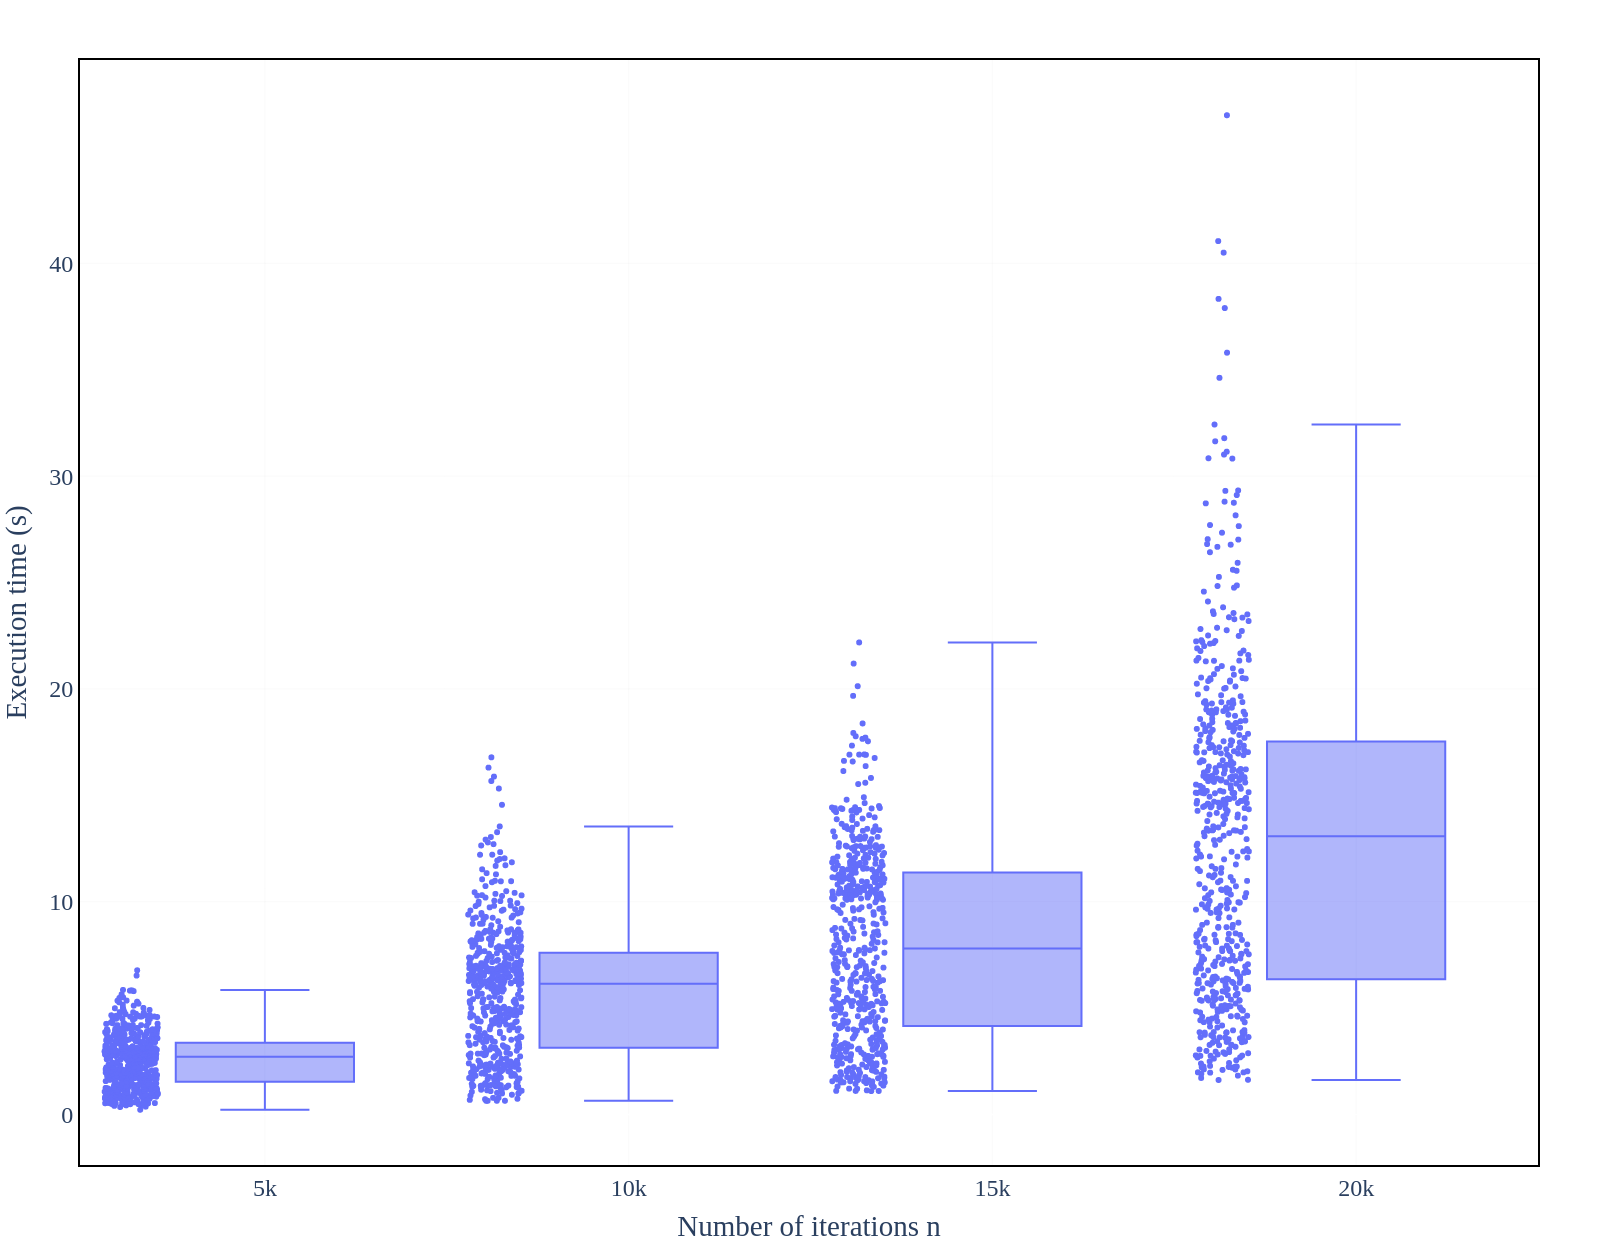
\includegraphics[width=\linewidth]{n_box_plot.png}
    \caption{Box-plot of the execution time (in seconds) with several values of $n$, for $p=4$. A linear dependance can be seen for the median.}
    \label{fig:benchmark-n_bplot}
\end{figure}
\begin{figure}[h]
    \centering
    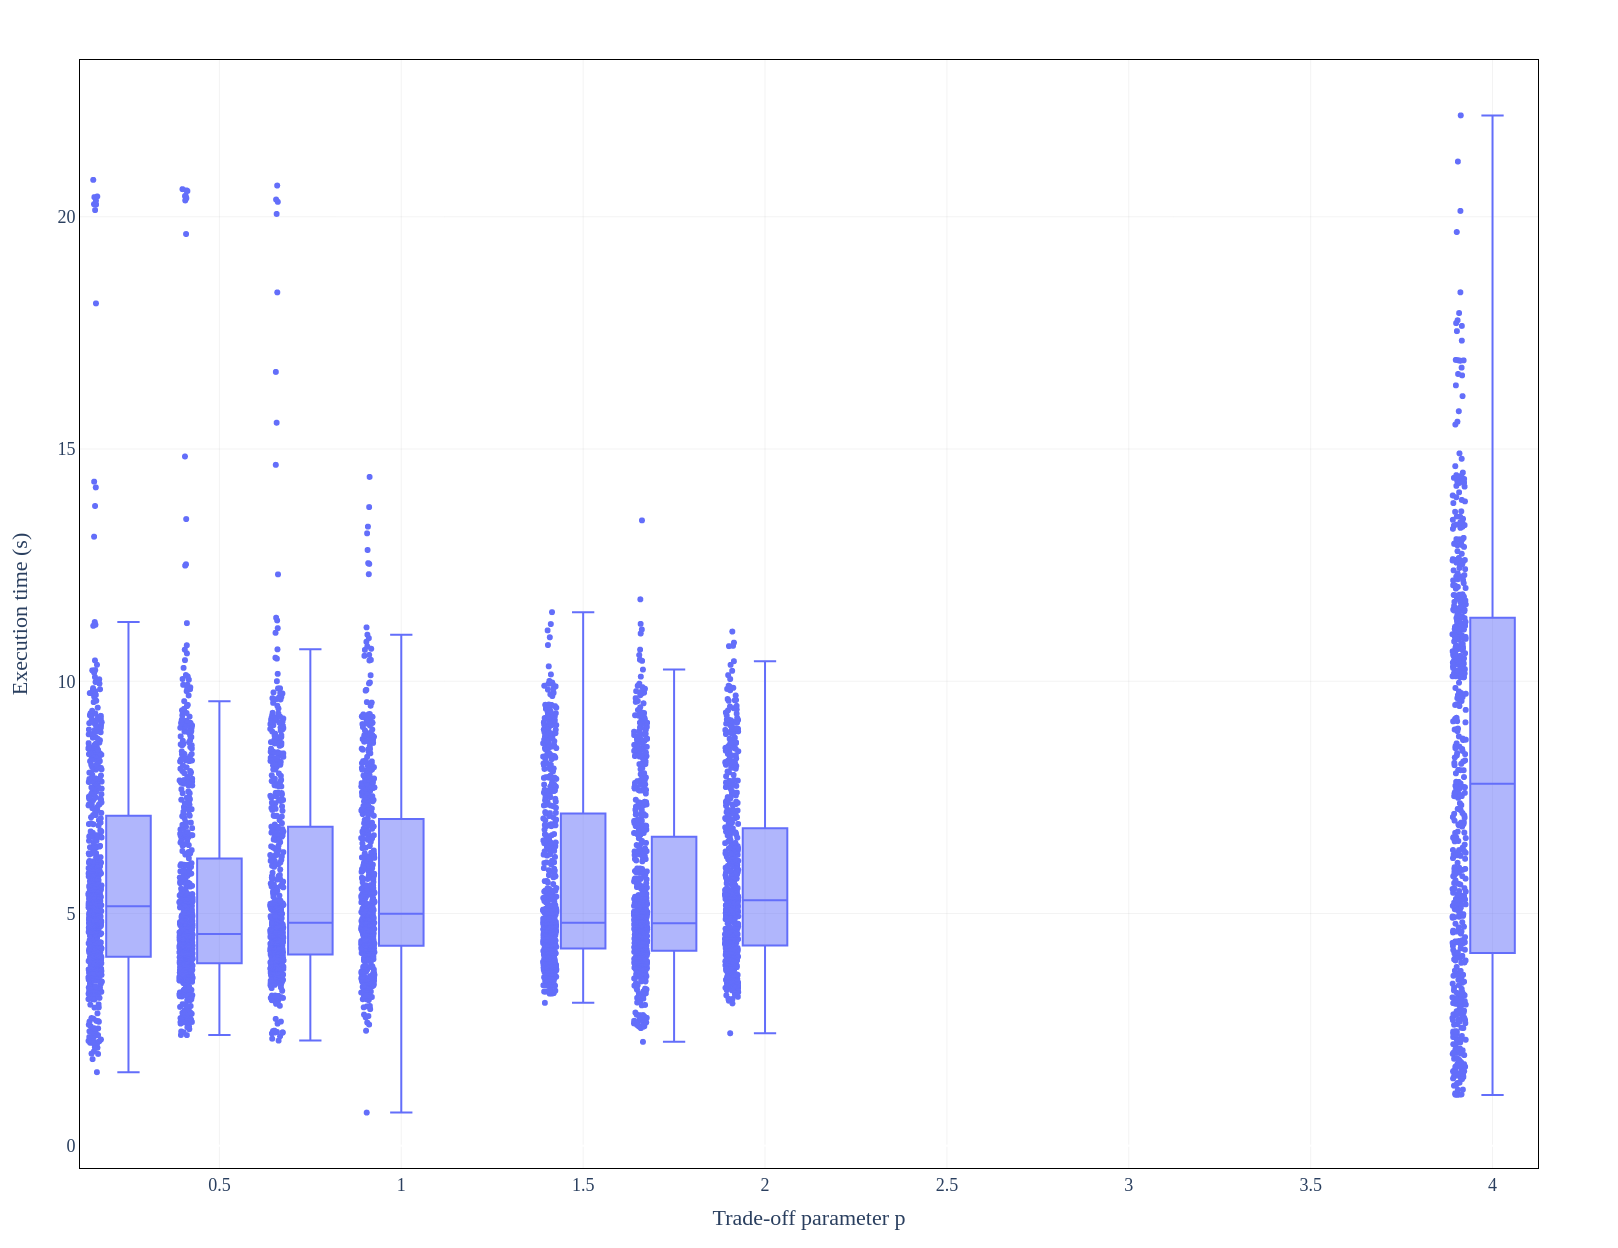
\includegraphics[width=\linewidth]{p_box_plot.png}
    \caption{Box-plot of the execution time (in seconds) with several values of $p$, for $n=15k$. As expected, the average execution time does not depend on $p$, hence is constant, although it seems like the execution time seems to spread for high $p$.}
    \label{fig:benchmark-p_bplot}
\end{figure}

\subsection{Evolution of the computation time through games}
Tweaking the settings of MCTS or minimax could in theory allow to reach equivalent results as minimax but these would not be achieved using the same computation time.
This section explores this idea by comparing the evolution of this time for both algorithms.

As Monte Carlo Tree Search simulates a game to its end at each iteration it is reasonable to think that the computation
time of each move will decrease during the game.
As the end approaches, the number of moves to simulate decreases.
Minimax on the other hand should use a more uniform time during the game since it is a simple tree exploration up to a certain depth (with pruning which will on average offer a constant improvement)
It could be interesting to see if the time of MCTS ends up better than the one of minimax, and if so around which turn it happens.
This could allow to use both algorithms at their best.

Figure~\ref{fig:benchmark-time_turn} shows this evolution.
One can notice that as expected the compution time of MCTS decreases with time, by a factor of almost four from the beginning to the end of the game.
Most of this evolution happens in the first twenty-five moves. 
However, minimax times are so low (for similar final results) that mcts never reaches them. 
Improvements in the implementation could change this as mentioned in section~\ref{sec:param_approach}.

\begin{figure}[ht]
    \centering
    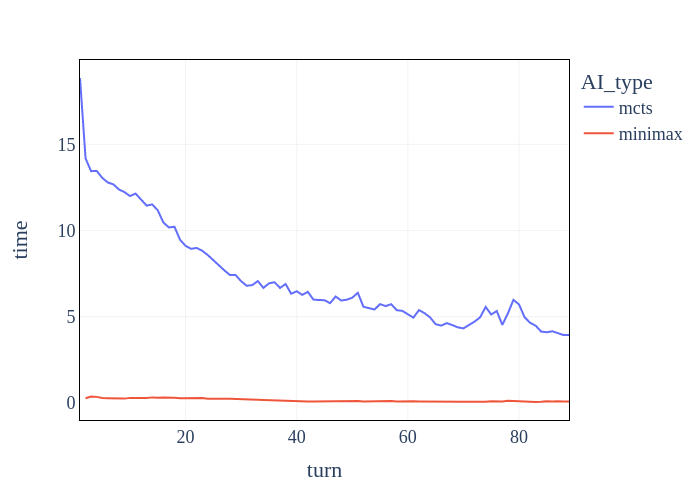
\includegraphics[width=\linewidth]{plots/AvgTime_n20000.png}
    \caption{Computing time [s] of both used algorithms (MCTS with $n=20k$) as a function of the number of turn played. MCTS diminishes but does not reach minimax in these settings. The dataset consists in about 80 games with $n=20k$ and 8 different parameters of $p$. However, as $p$ doesn't play a role in the execution time (as shown on figure \ref{fig:benchmark-p_bplot}), we can consider that the 80 games are indeed comparable in their execution times.}
    \label{fig:benchmark-time_turn}
\end{figure}

\subsection{Number turns in a time t}
In order to continue the exploration of the combination of minimax and MCTS started in the previous section,
a histogram was made to compare the number of turns in a certain time for minimax and MCTS. This histogram can
be found on the figure~\ref{fig:histo}.\\

The graph presented earlier gives you an idea of what the histogram will look like. Indeed, the minimax rounds always take less time than those made by MCTS.
The time taken per minimax is always between 1 and 3 seconds. By the way, on the histogram, some times look negative but this is simply the distribution chosen for the buckets used.
The minimax algorithm is much more stable than MCTS, the times are concentrated in the first two buckets of the histogram. For MCTS, the time taken for the rounds changes a lot.
A peak is reached between 7 and 9 seconds, i.e. more than 3 times the average time for minimax.

However, the number of laps that take more than 15 seconds is quite low compared to the rest. Even though MCTS takes longer than minimax,
this time is still reasonable and considering that this algorithm may be more efficient at the beginning of a game, it would certainly be advantageous to use both algorithms.

\begin{figure}[ht]
    \centering
    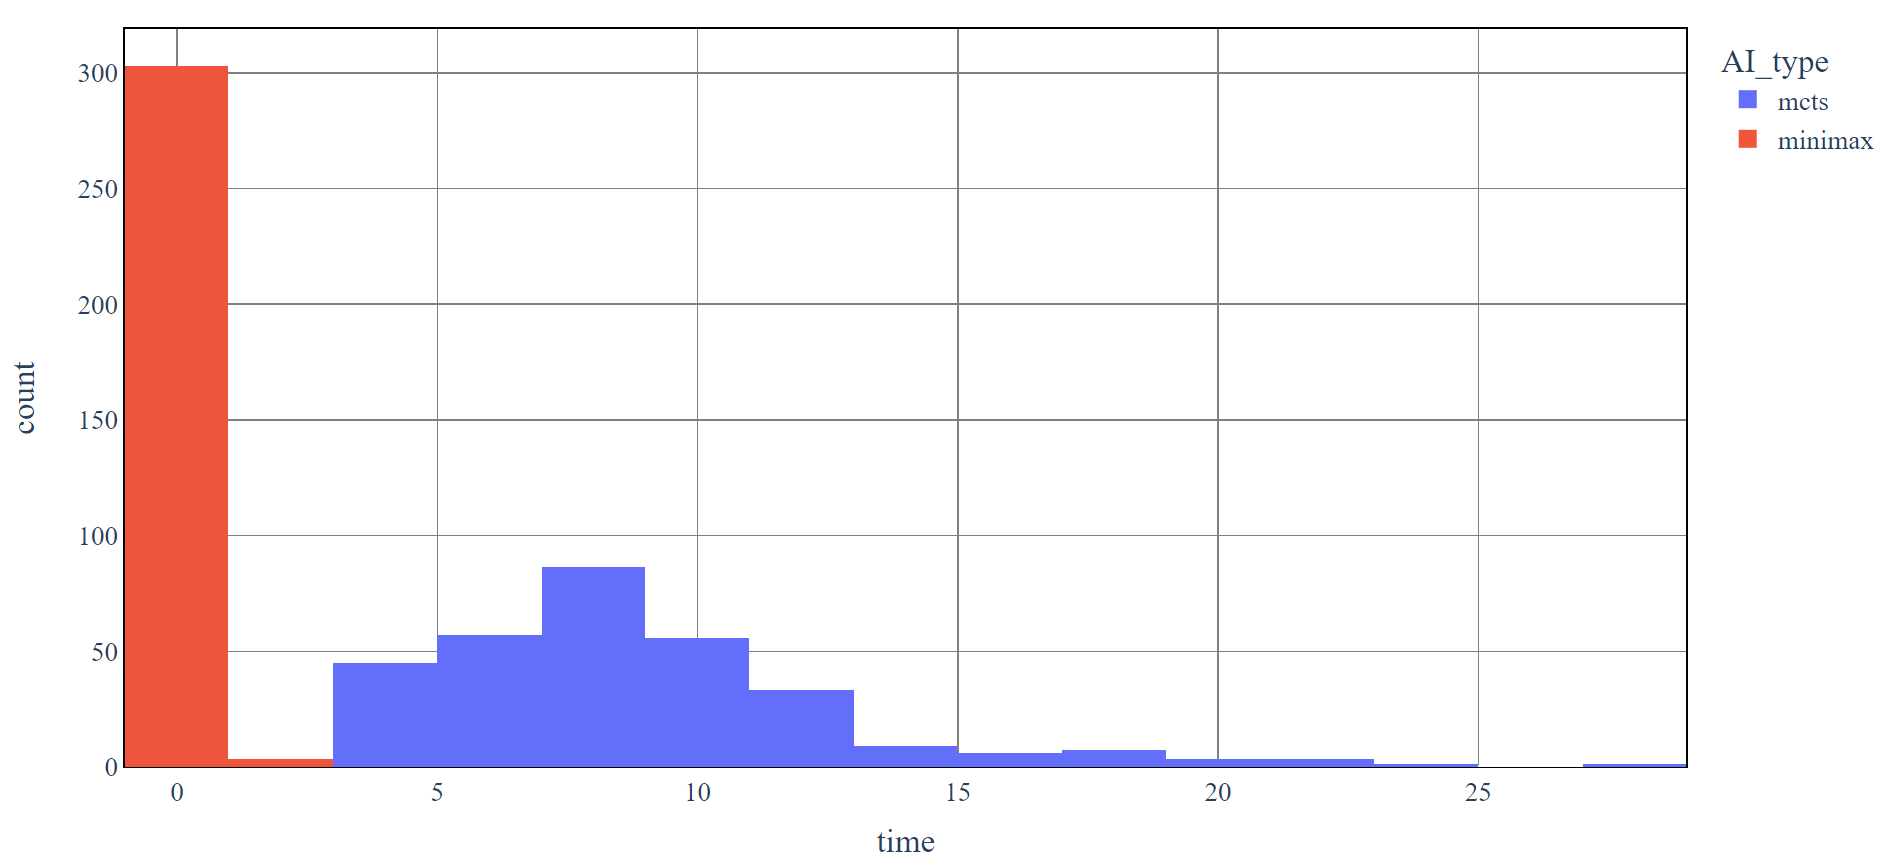
\includegraphics[width=\linewidth]{nb_turn_in_time_t.png}
    \caption{Histogram of number of turns of both used algorithms that take a certain time [s].}
    \label{fig:histo}
\end{figure}

\begin{appendices}
\section{Listings}
\begin{lstlisting}[language=python, label=listing:constructor, caption={Constructor of a Monte-Carlo Tree-Search Node}]
    class MCNode:
        def __init__(self, state: Board, color, nb_king_moved, max_it, parent=None, move: Move = None):
            self.state: Board = state
            self.color = color
            self.adv_color = WHITE if self.color == RED else RED
            self.reward = 0
            self.visits = 1  # We always visit newly created node
            self.parent = parent
            self.parent_action = move
            self.children: List[MCNode] = []
            self.children_moves = []
            self.max_it = max_it
            self.nb_king_moved = nb_king_moved  # To keep a track to see if the game needs to end
            return
    \end{lstlisting}

    
    \begin{algorithm}
    \caption{Selection of a node. Calls the \term{Best Child policy} and the \term{Expansion} procedure.}\label{listing:selection}
    \begin{algorithmic}
        \Procedure{select}{$N$}
        \State $N$\Comment{MC Root Node}
        \State CurrentNode = $N$ 
        \While {CurrentNode is not leaf} 
        \If 
        {CurrentNode is not fully explored} 
        \State \Return CurrentNode.\term{Expand}()
        \Else 
        \State CurrentNode = \term{BestChild}(CurrentNode)
        \EndIf
        \EndWhile
        \EndProcedure
    \end{algorithmic}
\end{algorithm}
²
\begin{algorithm}
    \caption{Expansion of a node}\label{listing:expand}
    \begin{algorithmic}
    \Procedure{expand}{$N$}
    \State $N$\Comment{Current MC Node}
    \State $r = $ random(RemainingMoves(N))
    \State newBoard = $N$.board.simulateMove($r$)
    \State $N_r = $ MCNode($N$, $r$, newBoard)
    \State \Return $N_r$
    \EndProcedure
    \end{algorithmic}
\end{algorithm}
\end{appendices}
\end{document}
